\section{Experimental Studies}
\label{sec:experiments}

% NOTE: This section is written for the main paper. It emphasizes the empirical
% claims and defers implementation details to the appendix file
% paper/experiments_appendix.tex.

\subsection{Synthetic Experiment}
\label{subsec:synthetic-experiments}

\paragraph{Setup.}
We first use frozen-teacher linear experiments with known population operators
to isolate the mechanisms in the theory from nonlinear optimization effects.
Full setup details are in \cref{app:synthetic-experimental-details}.

\paragraph{Models and baselines.}
The learned model is the finite-sample RRR solution. Rank $d$ instantiates the
JEPA bottleneck. Population operators and unconstrained OLS serve as baselines.

\paragraph{Metrics.}
Risk panels use the per-target normalization in \eqref{eq:per_target_risk}.
Diagnostics match the quantities in \cref{thm:unified_risk_decomposition} and
the rank, heterogeneity, and conditioning results. Definitions are in
\cref{app:synthetic-experimental-details}.

\paragraph{Results.}
The appendix figures
\cref{fig:k-saturation,fig:heterogeneity,fig:bottleneck} validate the
pre-saturation and bottleneck claims. Complementary target stacks increase
predictive rank, larger $\lambda_{\mathrm{het}}$ improves finite-sample
identifiability, and the rank-$d$ bottleneck induces the spectral-tail floor
predicted by \cref{prop:rank_growth,prop:heterogeneity_identifiability,prop:capacity_lower_bound}.
The main synthetic diagnostic is \cref{fig:post-saturation}. It tests
\cref{prop:post_saturation_risk} in the regime $r_\star(K)=d$, where
additional target blocks cannot create new rank. The experiment allocates new
blocks to weak predictive directions. As
$\kappa_K^2=\lambda_d(H_K)/\lambda_1(H_K)$ increases, the observed excess risk
and per-target risk decrease. \Cref{fig:predictive-isotropy} tests
\cref{lem:predictive_isotropy,thm:predictive_isotropy_opt}: at fixed rank and
trace, flatter spectra of $H_K=T_K^\top T_K$ improve recovery and reduce the
balanced-reference-stack excess risk. The gauge-factorization diagnostic in
\cref{fig:gauge-factorization} checks that the encoder-isotropy claims in
\cref{subsubsec:gauge_factorization} are factorization effects rather than new
end-to-end prediction constraints.

\begin{figure}[t]
    \centering
    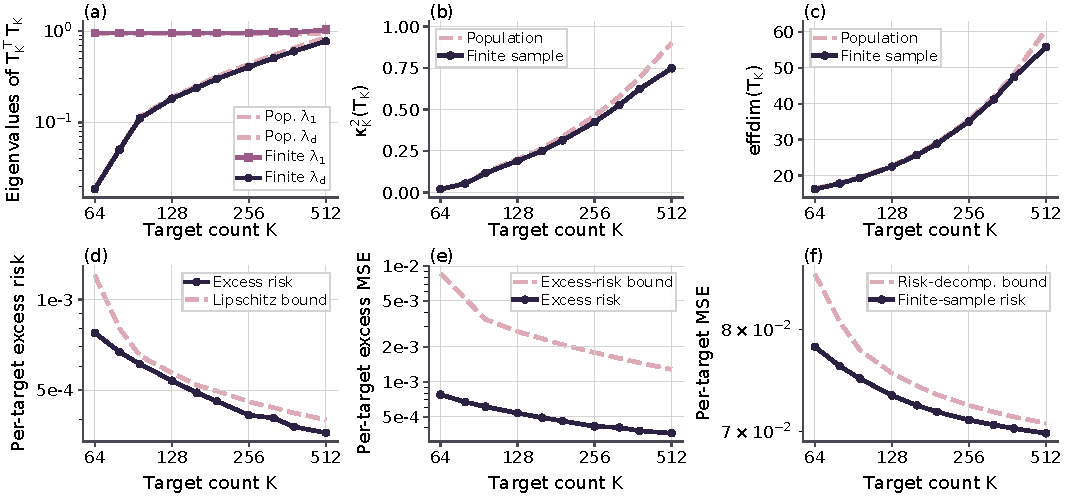
\includegraphics[width=0.97\linewidth]{figures/exp_post_saturation.pdf}
    \vspace{-0.6em}
    \caption{\small \textbf{Post-saturation conditioning.} Given $r_\star(K)=d$,
    allocating targets to weak directions increases $\kappa_K^2$ and reduces
    excess risk and per-target risk.
    Panel (d) plots the calibrated Lipschitz bound
    $\widehat L\|\sin\Theta_T\|_{\mathrm{op}}$.}
    \label{fig:post-saturation}
    \vspace{-2em}
\end{figure}

\subsection{Realistic Experiment}
\label{subsec:realistic-regularizer-experiments}

\paragraph{Setup.}
We test the practical regularizer~\eqref{eq:predictive_isotropy_regularizer}
in learned nonlinear image inpainting tasks. In both tasks the context is the
left half of a digit image and the target is the right half.
\Cref{fig:regularizer-mnist-cnn-samples} shows the task.

\paragraph{Data.}
The small-data diagnostic uses the \texttt{sklearn} $8\times8$ digit dataset.
The scaled diagnostic uses standard $28\times28$ MNIST. All pixels are
normalized to $[0,1]$.

\paragraph{Models.}
The small-data task uses an MLP encoder-predictor, and MNIST uses a
convolutional encoder-decoder. The prediction-side regularizer is applied to
the predictor representation as in \eqref{eq:predictive_isotropy_regularizer};
architecture and optimizer details are in
\cref{app:real-image-regularizer-details}.

\paragraph{Baselines.}
We compare four objectives: no regularization, Encoder Gaussianity,
prediction-side Gaussianity, and their combination. Encoder Gaussianity is the
standard representation-side control. Prediction-side Gaussianity is our
theory-motivated regularizer in
\eqref{eq:predictive_isotropy_regularizer}, and the combined objective is an
ablation testing whether Encoder Gaussianity improves on prediction-side
Gaussianity.

\paragraph{Metrics.}
We report target-half pixel MSE and RMSE. For MNIST we also
report foreground MSE, computed on non-background right-half pixels as most
right-half pixels are background. Gaussianity and effective-rank diagnostics are
reported in \cref{fig:regularizer-digits,fig:regularizer-mnist}; prediction
risk is the primary outcome.

\paragraph{Results.}
\Cref{fig:regularizer-mnist-cnn-samples} visualizes the digit-half prediction task,
and \cref{tab:regularizer-realdata} reports the regularizer
diagnostics. Additional completion examples are shown in
\cref{fig:regularizer-digits-samples,fig:regularizer-mnist-mlp-samples}. On
the low-label $8\times 8$ digit task, prediction-side
regularization reduces test MSE from $9.23{\times}10^{-2}$ to
$6.00{\times}10^{-2}$ and train--test gap from $8.54{\times}10^{-2}$ to
$2.00{\times}10^{-2}$. On the scaled MNIST task, prediction-side regularization
improves test MSE from $3.68{\times}10^{-2}$ to $3.43{\times}10^{-2}$ and
foreground MSE from $1.29{\times}10^{-1}$ to $1.19{\times}10^{-1}$. The
combined objective adds little, consistent with the subsumption view in
\cref{thm:subsumes_cov_isotropy,thm:subsumes_gaussian_isotropy}.

\begin{table}[t]
\centering
\caption{\small \textbf{Real-image regularizer diagnostics.} MSE and gap columns are reported in
$10^{-2}$ units, and RMSE is reported as a percentage of the normalized $[0,1]$
pixel range. Gap is test MSE minus train MSE. Foreground MSE is reported only
for MNIST, where background pixels dominate the right-half target.}
\label{tab:regularizer-realdata}
% \vspace{-0em}
\scriptsize
\setlength{\tabcolsep}{2pt}
\begin{tabular}{llccccc}
\hline
Task & Objective & Test MSE & RMSE (\%) & Test/Train Gap & FG MSE & Time \\
\hline
$8{\times}8$ digits & No reg. &
$9.23{\pm}0.17$ &
$30.4{\pm}0.3$ &
$8.54{\pm}0.17$ &
- &
$9.03{\pm}0.20$ s \ $(1.00{\times})$ \\
$8{\times}8$ digits & Enc. reg. &
$7.86{\pm}0.13$ &
$28.0{\pm}0.2$ &
$6.29{\pm}0.14$ &
- &
$12.55{\pm}0.11$ s \ $(1.39{\times})$ \\
$8{\times}8$ digits & Pred. reg. &
$\mathbf{6.00{\pm}0.03}$ &
$\mathbf{24.5{\pm}0.1}$ &
$\mathbf{2.00{\pm}0.07}$ &
- &
$12.23{\pm}0.04$ s \ $(1.35{\times})$ \\
$8{\times}8$ digits & Pred.+Enc. &
$6.09{\pm}0.04$ &
$24.7{\pm}0.1$ &
$2.27{\pm}0.08$ &
- &
$15.80{\pm}0.13$ s \ $(1.75{\times})$ \\
\hline
MNIST CNN & No reg. &
$3.68{\pm}0.02$ &
$19.19{\pm}0.04$ &
$2.81{\pm}0.05$ &
$12.90{\pm}0.07$ &
$69.52{\pm}4.23$ s \ $(1.00{\times})$ \\
MNIST CNN & Enc. reg. &
$3.65{\pm}0.02$ &
$19.11{\pm}0.05$ &
$2.68{\pm}0.05$ &
$12.75{\pm}0.07$ &
$55.39{\pm}0.13$ s \ $(0.80{\times})$ \\
MNIST CNN & Pred. reg. &
$\mathbf{3.43{\pm}0.02}$ &
$\mathbf{18.53{\pm}0.04}$ &
$2.13{\pm}0.06$ &
$\mathbf{11.92{\pm}0.06}$ &
$53.98{\pm}0.07$ s \ $(0.78{\times})$ \\
MNIST CNN & Pred.+Enc. &
$3.47{\pm}0.01$ &
$18.63{\pm}0.04$ &
$\mathbf{2.12{\pm}0.05}$ &
$12.06{\pm}0.05$ &
$39.08{\pm}4.30$ s \ $(0.56{\times})$ \\
\hline
\end{tabular}
    \vspace{-1.5em}
\end{table}

\begin{figure}[t]
    \centering
    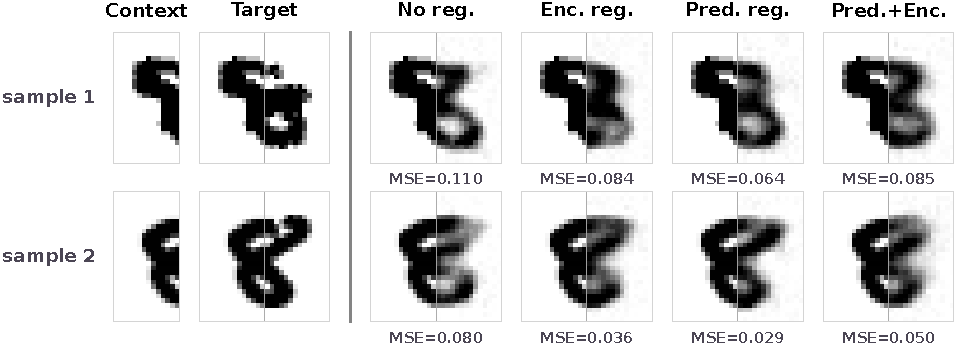
\includegraphics[width=0.8\linewidth]{figures/exp_regularizer_mnist_gpu_samples.pdf}
    \vspace{-0.8em}
    \caption{\small \textbf{MNIST half-completions.} Rows are held-out samples; columns show
    context, ground truth, and candidate completions. Cell labels report
    per-sample target-half pixel MSE.}
\label{fig:regularizer-mnist-cnn-samples}
\vspace{-1.8em}
\end{figure}
